% Author: Santiago Faci <santiago.faci@gmail.com>
% www.videosdeinformatica.com

\documentclass[xcolor={dvipsnames}]{beamer}
\setbeamertemplate{navigation symbols}{}

\usepackage{beamerthemeshadow}
\usepackage[spanish]{babel}
\usepackage{url}
\usepackage[utf8]{inputenc}

\definecolor{resalta}{cmyk}{0,1,0,0}

\usepackage{listings}
\lstset{basicstyle=\tiny\ttfamily,breaklines=true}
\lstset{framextopmargin=50pt}
\lstset{keywordstyle=\tiny\color{blue}\bfseries}
\lstset{stringstyle=\tiny\color{red}\ttfamily}
\lstset{commentstyle=\tiny\color{OliveGreen}\ttfamily}
\lstset{showstringspaces=false}

\begin{document}
\title{Taller de Desarrollo de Aplicaciones con Android}  
\author{Santiago Faci}
\institute{Centro Afuera}
\date{Junio 2019} 

\begin{frame}
\titlepage
\end{frame}

\begin{frame}[plain]\frametitle{Índice}\tableofcontents
\end{frame} 


\section{¿Qué es Android?} 
\begin{frame}\frametitle{¿Qué es un framework?} 
    \begin{block}{framework}
    Un framework es un conjunto de programas, bibliotecas, lenguajes y otras herramientas, que sirve de base para el desarrollo de software.
    \end{block}
    \begin{block}{}
    En función del framework utilizado, se creará un tipo u otro de aplicación
    \end{block}
\end{frame}

\begin{frame}\frametitle{Android Framework / Sistema Operativo}
    \begin{block}{Android SDK}
    Android SDK es el kit de desarrollo que permite crear aplicaciones para este Sistema Operativo

    Android SDK funciona como un framework que, utilizando lenguaje Java, permite desarrollar aplicaciones apoyándose en multitud de librerías y
    herramientas ya creadas con una estructura definida.
    \end{block}
    \pause \begin{block}{Android Sistema Operativo}
    Android es además un Sistema Operativo (basado en Linux) para dispositivos móviles (tablets, smartphones, smartwatches, \ldots) que viene
    instalado en numerosos terminales
    \end{block}
\end{frame}

\section{Estructura de Android} 
\subsection{Estructura del Sistema Operativo}
\begin{frame}\frametitle{Estructura de Android}
    \begin{figure}
    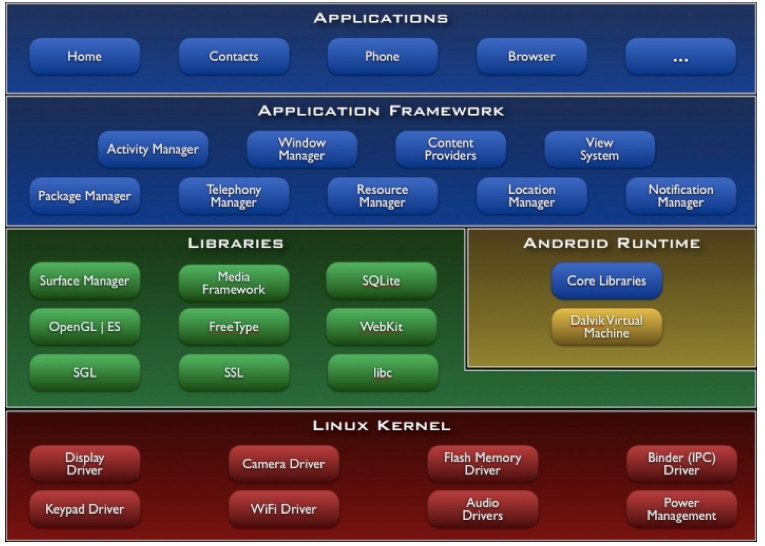
\includegraphics[scale=0.28]{images/estructura_android} 
    \caption{Framework Android}
    \end{figure}
\end{frame}

\subsection{Ciclo de vida de una aplicación}
\begin{frame}[plain]\frametitle{Ciclo de vida de una aplicación Android}
    \begin{figure}
    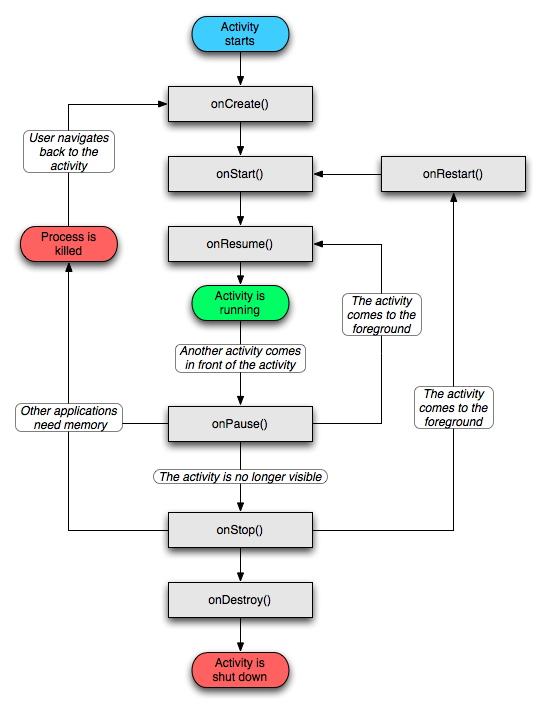
\includegraphics[scale=0.3]{images/activity_lifecycle} 
    %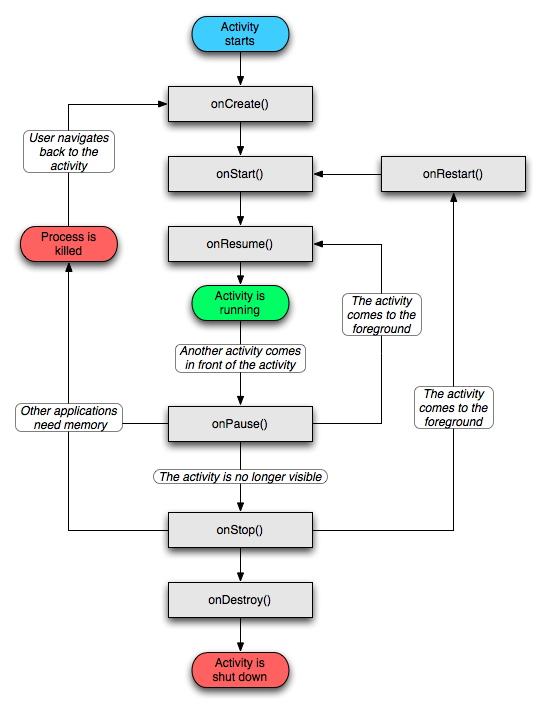
\includegraphics[width=\paperwidth,height=\paperheight]{images/activity_lifecycle} 
    \caption{Ciclo de vida}
    \end{figure}
\end{frame}

\subsection{Estructura de una Aplicación}
\begin{frame}\frametitle{Estructura del proyecto}
    \begin{columns}
        \begin{column}{4cm}
        \begin{figure}
        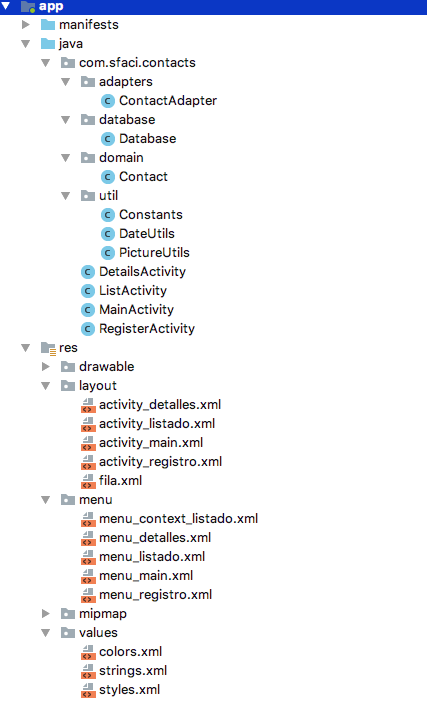
\includegraphics[scale=0.2]{images/project_structure} 
        \caption{Proyecto Android}
        \end{figure}
        \end{column}
        \pause
        \begin{column}{6cm}
        \begin{block}{}
        \begin{itemize}
            \item \emph{\textcolor{resalta}{java}} Código de aplicación
            \item \emph{\textcolor{resalta}{res}} Recursos del proyecto
            \item \emph{\textcolor{resalta}{drawable}} Iconos de la aplicación
            \item \emph{\textcolor{resalta}{layout}} Diseño de las pantallas
            \item \emph{\textcolor{resalta}{menu}} Diseño de los diferentes menús
            \item \emph{\textcolor{resalta}{values}} Recursos de texto
            \item \emph{\textcolor{resalta}{manifests}} Almacena el manifiesto del proyecto con la configuración general del mismo
        \end{itemize}
        \end{block}
        \end{column}
        \end{columns}
    \end{frame}

\begin{frame}\frametitle{Recursos de aplicación}
    \begin{block}{}
    Los recursos son todos aquellos ficheros que no forman parte del código de la aplicación. Se localizan dentro de la carpeta
    \emph{\textcolor{resalta}{res}}
    en la estructura del proyecto y se distribuyen a su vez en carpetas
    \end{block}
    \begin{itemize}
        \pause \item \emph{\textcolor{resalta}{drawable}} Repetida con algunos de estos sufijos (\emph{xhdpi}, \emph{hdpi}, \emph{ldpi}, \emph{mdpi}),
        almacena los recursos gráficos del proyecto en sus diferentes resoluciones (según sufijo)
        \pause \item \emph{\textcolor{resalta}{layout}} Diseños de las diferentes pantallas de la aplicación
        \pause \item \emph{\textcolor{resalta}{values}} Cualquier otro recurso que no sea código (textos de la aplicación, opciones, . . .)
        \pause \item \emph{\textcolor{resalta}{menu}} Diseño de los menús de la aplicación
    \end{itemize}
\end{frame}

\begin{frame}\frametitle{Código de aplicación}
    \begin{block}{Código desarrollado}
    El código desarrollado se empaqueta como una aplicación \emph{Java}.
    \end{block}
    \begin{block}{Código generado}
    Todos los recursos del proyecto generan, automáticamente, una clase \emph{\textcolor{resalta}{R}} para utilizar éstos desde el código de la aplicación
    \end{block}
\end{frame}

\begin{frame}[fragile]\frametitle{Fichero de manifiesto I}
    \begin{block}{}
    \begin{lstlisting}[language=XML]
<manifest xmlns:android="http://schemas.android.com/apk/res/android"
          package="org.sfaci.helloworld"
          android:versionCode="1"
          android:versionName="1.0">
    \end{lstlisting}
    \end{block}
    \begin{block}{}
    Define el paquete base de la aplicación y el número y nombre de versión de la misma
    \end{block}
\end{frame}

\begin{frame}[fragile]\frametitle{Fichero de manifiesto II}
    \begin{block}{}
    \begin{lstlisting}[language=XML]
<uses-sdk android:minSdkVersion="18"/>
    \end{lstlisting}
    \end{block}
    \begin{block}{}
    Indica la versión mínima de Android (\emph{API Level}) soportada por la aplicación (requisitos mínimos para funcionar)
    \begin{itemize}
        \item Android 2.3.3 $\rightarrow$ \emph{API Level 10}
        \item Android 3.0 $\rightarrow$ \emph{API Level 11}
        \item \ldots
        \item Android 4.3 $\rightarrow$ \emph{API Level 18}
        \item Adnroid 4.4 $\rightarrow$ \emph{API Level 19}
    \end{itemize}
    \end{block}
\end{frame}

\begin{frame}[fragile]\frametitle{Fichero de manifiesto III}
    \begin{block}{}
    \begin{lstlisting}[language=XML]
<application android:label="@string/app_name" android:icon="@drawable/ic_launcher">
    \end{lstlisting}
    \end{block}
    \begin{block}{}
    Define el nombre de la aplicación y su icono
    \end{block}
\end{frame}

\begin{frame}[fragile]\frametitle{Fichero de manifiesto IV}
    \begin{block}{}
    \begin{lstlisting}[language=XML]
<activity android:name="MyActivity"
          android:label="@string/app_name">
    <intent-filter>
        <action android:name="android.intent.action.MAIN"/>
        <category android:name="android.intent.category.LAUNCHER"/>
    </intent-filter>
</activity>
    \end{lstlisting}
    \end{block}
    \begin{block}{}
    \begin{itemize}
        \item Define cada una de las \emph{Activity} que componen la aplicación
        \item Solamente una se debe definir como \emph{Activity} principal (la del ejemplo en este caso)
    \end{itemize}
    \end{block}
\end{frame}

\begin{frame}\frametitle{Empaquetado de la aplicación}
    \begin{block}{}
    El empaquetado de la aplicación lo realiza la propia aplicación generando un fichero .apk que se puede instalar directamente en
    cualquier móvil Android.
    \end{block}
    \begin{itemize}
        \item Cada vez que ejecutamos la aplicación sobre el emulador o nuestro dispositivo para depurar, se genera automáticamente una
        versión empaquetada de la misma que sólo puede ser utilizada para esos fines.
        \item Se debe firmar con nuestro fichero de claves si queremos distribuir la aplicación y subirla a Google Play.
    \end{itemize}

\end{frame}

\begin{frame}\frametitle{Mapas}
    \begin{block}{}
    Se pueden utilizar muchas de las librerías existentes, además de Google Maps. En este caso utilizaremos la librería Mapbox, que podemos
    usar gratuitamente mientras nuestra aplicación no supere los 25.000 usuarios activos mensuales o las 50.000 cargas mensuales de mapas.
    \end{block}
    \begin{itemize}
        \item Disponible en \emph{http://www.mapbox.com} 
    \end{itemize}

\end{frame}

\section{Acceso a Bases de Datos}
\subsection{SQLite}
\begin{frame}\frametitle{¿Qué es SQLite?}
    \begin{itemize}
        \item Motor de Base de Datos de tamaño muy reducido (unos pocos MB)
        \item Ideal para Bases de Datos \emph{pequeñas} (aprox. 1 GB)
        \item Perfecto para pequeños dispositivos
        \item No necesita instalación (un único fichero .jar en el caso de Java)
        \item Viene \emph{de serie} con Android
        \item Fácil de usar (sólo hay que saber \emph{SQL} y manejarse con \emph{JDBC})
        \item Muchas aplicaciones lo usan (\emph{Whatsapp}, por ejemplo)
    \end{itemize}
\end{frame}

\end{document}
